% The tour figure for \S2. Kept in its own file so it can be redrawn without touching main.tex.
% Encoding: red is what Rio actually does, black is the pol-level narration of it,
% dashed is the route not taken, and shading is freshly built material (as in \cref{fig:planner-add-vs-replace}).
\definecolor{actcol}{HTML}{D55E00}
% \opicon: the operator, at text size. Presence marks a policy someone wrote.
\newcommand{\opicon}{%

\begin{tikzpicture}[baseline=-0.35ex, x=1ex, y=1ex]
  \fill[black!62] (0,0.78) circle (0.46);
  \fill[black!62] (-0.86,-1.05) .. controls (-0.86,0.22) and (0.86,0.22) .. (0.86,-1.05) -- cycle;
\end{tikzpicture}}

\begin{figure*}[t]
\centering
  \begin{tikzpicture}[
    >={Stealth[length=4.5pt]},
    polbox/.style={draw=black!30, rounded corners=2.5pt, inner sep=5.5pt, anchor=north},
    ctlbox/.style={draw=black!30, rounded corners=2.5pt, fill=black!4,
                   inner xsep=7pt, inner ysep=4.5pt, anchor=north, font=\scriptsize},
    hd/.style={font=\scriptsize, inner sep=2pt, anchor=south},
    sem/.style={font=\scriptsize, inner sep=1.5pt},
    act/.style={sem, text=actcol},
    gd/.style={font=\scriptsize\itshape, text=black!55, inner sep=1.5pt, align=center},
    does/.style={draw=actcol, line width=1.1pt},
    says/.style={draw=black!75, line width=0.6pt},
    notaken/.style={draw=black!45, line width=0.6pt, dashed},
  ]
  % anchor=center is load-bearing on pn: a panel is a tikzpicture inside a \node, and
  % that node's anchor leaks in, so without it every label hangs off the corner named
  % by its own panel's polbox and the triangles come out crooked.
  % Uniform text height/depth keeps .north on one line per level whatever the glyphs.
  \tikzset{
    pn/.style={font=\scriptsize, inner sep=1pt, anchor=center,
               text height=1.7ex, text depth=0.5ex},
    edge/.style={shorten >=1.2pt, shorten <=0.5pt},
    el/.style={font=\scriptsize, inner sep=0.8pt, text=black!55},
  }

  % ============================ p_1 ============================
  \node[polbox, anchor=north west] (P1) at (0,0) {%
  \begin{tikzpicture}[x=1cm,y=1cm]
    \node[pn] (a0) at ( 0.00, 0)     {\(\Strict\)};
    \node[pn] (a1) at (-0.98,-0.80)  {\textsf{zoom}};
    \node[pn] (a2) at ( 0.98,-0.80)  {\textsf{gmail}};
    \draw[edge] (a0.south) -- (a1.north) node[el, midway, above=1pt, xshift=-2pt] {hi};
    \draw[edge] (a0.south) -- (a2.north) node[el, midway, above=1pt, xshift=2pt] {lo};
  \end{tikzpicture}};

  % ==================== transitionary policy ====================
  \node[polbox] (P2) at (8.45,0) {%
  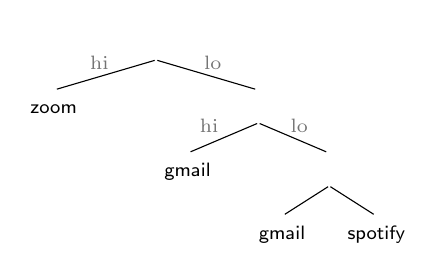
\begin{tikzpicture}[x=1cm,y=1cm]
    \node[pn] (b0)  at ( 0.00, 0.00) {\(\Strict\)};
    \node[pn] (b1)  at (-1.30,-0.80) {\textsf{zoom}};
    \node[pn] (b2)  at ( 1.30,-0.80) {\(\Strictstar\)};
    \node[pn] (b3)  at ( 0.40,-1.60) {\textsf{gmail}};
    \node[pn] (rr)  at ( 2.20,-1.60) {\(\RR\)};
    \node[pn] (rrA) at ( 1.60,-2.40) {\textsf{gmail}};
    \node[pn] (rrB) at ( 2.80,-2.40) {\textsf{spotify}};
    \draw[edge] (rr.south) -- (rrA.north);
    \draw[edge] (rr.south) -- (rrB.north);
    \freshbehind{(b2)}
    \freshbehind{(rr)(rrA)(rrB)}
    \draw[edge] (b0.south) -- (b1.north) node[el, midway, above=1pt, xshift=-2pt] {hi};
    \draw[edge] (b0.south) -- (b2.north) node[el, midway, above=1pt, xshift=2pt] {lo};
    \draw[edge] (b2.south) -- (b3.north) node[el, midway, above=1pt, xshift=-5pt] {hi};
    \draw[edge] (b2.south) -- (rr.north) node[el, midway, above=1pt, xshift=2pt] {lo};
  \end{tikzpicture}};

  % ============================ p_2 ============================
  \node[polbox, anchor=north east] (P3) at (17.5,0) {%
  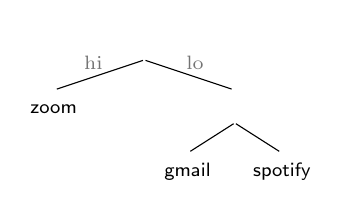
\begin{tikzpicture}[x=1cm,y=1cm]
    \node[pn] (d0)  at ( 0.00, 0.00) {\(\Strict\)};
    \node[pn] (d1)  at (-1.15,-0.80) {\textsf{zoom}};
    \node[pn] (rr)  at ( 1.15,-0.80) {\(\RR\)};
    \node[pn] (rrA) at ( 0.55,-1.60) {\textsf{gmail}};
    \node[pn] (rrB) at ( 1.75,-1.60) {\textsf{spotify}};
    \draw[edge] (rr.south) -- (rrA.north);
    \draw[edge] (rr.south) -- (rrB.north);
    \freshbehind{(rr)(rrA)(rrB)}
    \draw[edge] (d0.south) -- (d1.north) node[el, midway, above=1pt, xshift=-2pt] {hi};
    \draw[edge] (d0.south) -- (rr.north) node[el, midway, above=1pt, xshift=2pt] {lo};
  \end{tikzpicture}};

  % ===== headings: the operator marks the two policies somebody wrote =====
  \node[hd] at (P1.north) {\opicon\;\(p_1\)};
  \node[hd] at (P2.north) {\emph{transitionary policy}};
  \node[hd] at (P3.north) {\opicon\;\(p_2\)};

  % ============================ controls ============================
  \node[ctlbox] (C1)  at (P1.south |- 0,-3.55) {\(C_1\)};
  \node[ctlbox] (C2m) at (P2.south |- 0,-3.55) {\emph{transitionary control}};
  \node[ctlbox] (C2)  at (P3.south |- 0,-3.55) {\(C_2\)};

  % ============ black: the pol-level narration of the path ============
  \draw[says,->] ($(P1.north east)+(0.10,-0.42)$) -- ($(P2.north west)+(-0.10,-0.42)$)
    node[sem, midway, above=0.5pt] {\(\psem{\Designate;\Quiesce}\)};
  \draw[says,->] ($(P2.north east)+(0.10,-0.42)$) -- ($(P3.north west)+(-0.10,-0.42)$)
    node[sem, midway, above=0.5pt] {\(\psem{\Undesignate}\)};

  % ================ red: what Rio actually does ================
  \draw[does,->] ($(C1.east)+(0.10,0)$) -- ($(C2m.west)+(-0.10,0)$)
    node[act, midway, above=1pt] {\(\csem{\Designate;\Quiesce}\)}
    node[gd, midway, below=1pt] {immediately};
  \draw[does,->] ($(C2m.east)+(0.10,0)$) -- ($(C2.west)+(-0.10,0)$)
    node[act, midway, above=1pt] {\(\csem{\Undesignate}\)}
    node[gd, midway, below=1pt] {once the doomed \textsf{gmail} drains};
  \draw[does,->] (P1.south) -- (C1.north)
    node[act, midway, anchor=east, xshift=-2pt] {\(\lceil \cdot \rceil\)};
  \draw[does,->] (C2m.north) -- (P2.south)
    node[act, midway, anchor=west, xshift=2pt] {\(\lfloor \cdot \rfloor\)};

  % ================ dashed: the route not taken ================
  \draw[notaken,->] (P3.south) -- (C2.north)
    node[gd, midway, anchor=east, xshift=-4pt] {what a recompile\\would have built};

  \end{tikzpicture}
  \caption{The \Replace{} transition of \cref{sec:tour}. Red is what Rio does, dashed is the route it does not take.}
  \label{fig:tour}
\end{figure*}
